\section{Thực hiện mạch nguồn}

\begin{figure}[H]
	\centering
	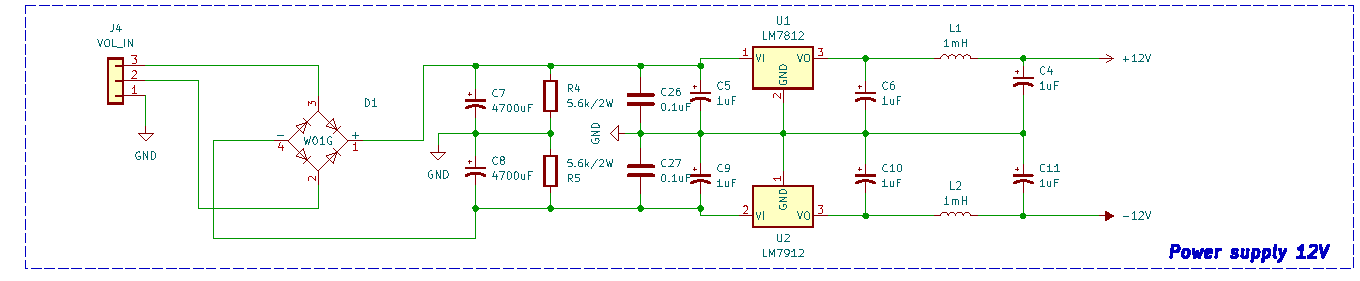
\includegraphics[width=.9\linewidth]{./my-chapters/my-images/Power_Source/power_supply.pdf}
	\caption{Tổng quan của mạch nguồn.}
\end{figure}

\subsection{Điện áp sau khi chỉnh lưu}

\begin{figure}[H]
	\centering
	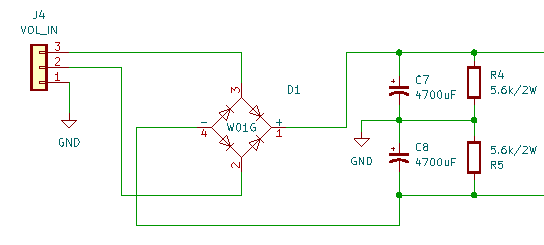
\includegraphics[width=0.6\linewidth]{./my-chapters/my-images/Power_Source/mach_chinh_luu.pdf}
	\caption{Mạch chỉnh lưu điện áp đầu vào.}
	\label{f_mach chinh luu}
\end{figure}

Giá trị VOL\_IN được cấp bởi đầu ra của biến áp với điện áp đầu ra của biến áp là $12VAC$, sau khi chỉnh lưu toàn sóng với tụ lọc là $C_7$ và $C_8$ thì điện áp ngõ ra của cầu diode được tính toán bằng công thức: \[V_{DC} = \sqrt{2}\times V_{AC} - 2\times V_{diode} \approx 15.6V\]
Trong đó, 
\begin{itemize}[label=-]
	\item $V_{DC}$: là điện áp ngõ ra sau khi chỉnh lưu toán sóng ($V$).
	\item $V_{AC}$: là điện áp ngõ vào cầu diode ($=12V$).
	\item $V_{diode}$: là sụt áp trên hai diode trong cầu chỉnh lưu ($=0.7V$).
\end{itemize}

Tụ $C_{7}$ và $C_{8}$ có chức năng làm giảm độ gợn sóng (ripple) và được tính bằng công thức: \[C = \dfrac{I}{f \times \Delta V} = 5000\mu F \approx 4700\mu F\]
Trong đó,
\begin{itemize}[label = -]
	\item $C$: là giá trị điện dung của tụ ($F$).
	\item $I$: là giá trị dòng tổng ($=1A$).
	\item $f$: là giá trị tần số sau khi chỉnh lưu ($=100Hz$).
	\item $\Delta V$: là độ gợn sóng mong muốn ($=2V$).
\end{itemize}

Điện trở $R_{4}$ và $R_{5}$ được gọi là \textit{Bleeder resistor} có tác dụng xả điện áp ở tụ $C_{7}$ và $C_{8}$ khi ngắt nguồn điện để đảm bảo an toàn cho hệ thống trong những trường hợp nguy hiểm xảy ra gây cho hai tụ này luôn nạp trong thời gian dài. Điện trở này sẽ có giá trị từ $2.2 \sim 10k\Omega$ và công suất từ $2 \sim 10W$.

\subsection{Điện áp cấp $+12V$}

\begin{figure}[H]
	\centering
	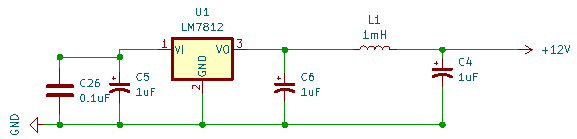
\includegraphics[width=0.6\linewidth]{./my-chapters/my-images/Power_Source/supply_+12V.pdf}
	\caption{Mạch cung cấp nguồn $+12V$.}
	\label{f_powersupply_+12V}
\end{figure}

Điện áp ngõ vào ($V_{in}$) của mạch cần phải đáp ứng tối thiểu theo công thức: \[ V_{in} > V_{out} + V_{dropout} = 12 + 2 = 14V \rightarrow V_{in} > 14V\]
Trong đó,
\begin{itemize}[label = -]
	\item $V_{in}$: là điện áp đầu vào ($V$).
	\item $V_{out}$: là điện áp đầu ra của LM7812 $=12V$.
	\item $V_{dropout}$: là điện áp rơi trên LM7812 $=2V$.
\end{itemize}

Công suất tiêu tán ($P_{loss}$) là công suất tiêu hao năng lượng dưới dạng nhiệt khi ổn áp: \[ P_{loss} = (V_{in} - V_{out}) \times I_{load} = (15.6 - 12)\times 1 = 3.6W\]
Trong đó,
\begin{itemize}[label=-]
	\item $P_{loss}$: là công suất tiêu tán trên LM7812 ($W$).
	\item $V_{in}$: là điện áp ngõ vào LM7812 ($=15.6V$).
	\item $V_{out}$: là điện áp ngõ ra LM7812 ($=12$).
	\item $I_{load}$: là dòng tải ($=1A$).
\end{itemize}

Kích thước tản nhiệt ($R_{th}$) để đảm bảo IC không quá nóng, nhiệt độ $T_j$ phải nằm trong giới hạn ($T_j \leq 125^{\circ}C$). Ta sử dụng công thức: \[ T_{j} = T_{o} + P_{loss} \times R_{th(tot)} \rightarrow R_{th(tot)} \leq \dfrac{T_{j} - T_{o}}{P_{loss}} = \dfrac{125 - 25}{3.6} \approx 27.8 \rightarrow R_{th(tot)} \leq 27.8^{\circ}C/W
\]
\[ \Rightarrow R_{th(c-a)} \leq R_{th(tot)} - R_{th(j-c)} = 27.8 - 5 \rightarrow R_{th(c-a)} \leq 22.8^{\circ}C/W \]
Trong đó,
\begin{itemize}[label = -]
	\item $T_{j}$: là nhiệt độ cho phép hoạt động của IC ($ ^\circ C$).
	\item $T_{o}$: là nhiệt độ của môi trường ($=25^{\circ}C$).
	\item $P_{loss}$: là công suất tiêu tán trên LM7812 ($=3.6W$).
	\item $R_{th(tot)}$: là tổng trở nhiệt từ junction đến môi trường ($27.8^{\circ}C/W$).
	\item $R_{th(j-c)}$: là trở nhiệt junction-to-case ($=5^{\circ}C/W$).
	\item $R_{th(c-a)}$: là trở nhiệt case-to-air ($^{\circ}C/W$).
\end{itemize}

Tụ điện đầu vào $C_{5}$ giúp bù sụt áp tạm thời và có giá trị là $1\mu F$.

Tụ điện đầu ra $C_{4}$ và $C_6$ giúp cải thiện ổn định điện áp đầu ra và có giá trị là $1\mu F$.

Tụ $C_{26}$ là tụ điện có chức năng dập nhiễu cao tần có giá trị là $0.1\mu F$.

Cuộn cảm $L_{1}$ có chức năng loại bỏ các nhiễu tần số cao có thể xuất hiện đầu ra, và tạo thành một bộ lọc LC giúp làm mịn điện áp đầu ra bằng cách giảm biên độ của các gợn sóng còn lại sau khi chỉnh lưu và ổn áp.

Hiệu suất ($\eta$) của mạch được tính bằng công thức: \[ \eta = \dfrac{V_{out}\times I_{load}}{V_{in} \times I_{load}}\times 100\% = \dfrac{12\times 1}{15.6 \times 1}\times 100\% \approx 76.9\% \]

\subsection{Điện áp cấp $-12V$}

\begin{figure}[H]
	\centering
	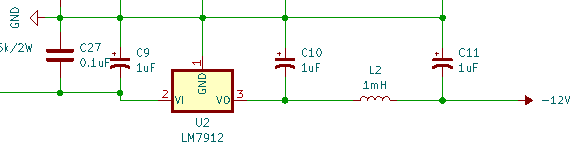
\includegraphics[width=0.6\linewidth]{./my-chapters/my-images/Power_Source/supply_-12V.pdf}
	\caption{Mạch cung cấp nguồn $-12V$.}
	\label{f_powersupply_-12V}
\end{figure}

Điện áp ngõ vào ($V_{in}$) của mạch cần phải đáp ứng tối thiểu theo công thức: \[ V_{in} < V_{out} - V_{dropout} = -12 - 2 = -14V \rightarrow V_{in} < -14V\]
Trong đó,
\begin{itemize}[label = -]
	\item $V_{in}$: là điện áp đầu vào ($V$).
	\item $V_{out}$: là điện áp đầu ra của LM7912 $=-12V$.
	\item $V_{dropout}$: là điện áp rơi trên LM7912 $=2V$.
\end{itemize}

Công suất tiêu tán ($P_{loss}$) là công suất tiêu hao năng lượng dưới dạng nhiệt khi ổn áp: \[ P_{loss} = (|V_{in}| - |V_{out}|) \times I_{load} = (15.6 - 12)\times 1 = 3.6W\]
Trong đó,
\begin{itemize}[label=-]
	\item $P_{loss}$: là công suất tiêu tán trên LM7912 ($W$).
	\item $V_{in}$: là điện áp ngõ vào LM7912 ($=-15.6V$).
	\item $V_{out}$: là điện áp ngõ ra LM7912 ($=-12$).
	\item $I_{load}$: là dòng tải ($=1A$).
\end{itemize}

Kích thước tản nhiệt ($R_{th}$) để đảm bảo IC không quá nóng, nhiệt độ $T_j$ phải nằm trong giới hạn ($T_j \leq 125^{\circ}C$). Ta sử dụng công thức: \[ T_{j} = T_{o} + P_{loss} \times R_{th(tot)} \rightarrow R_{th(tot)} \leq \dfrac{T_{j} - T_{o}}{P_{loss}} = \dfrac{125 - 25}{3.6} \approx 27.8 \rightarrow R_{th(tot)} \leq 27.8^{\circ}C/W
\]
\[ \Rightarrow R_{th(c-a)} \leq R_{th(tot)} - R_{th(j-c)} = 27.8 - 5 \rightarrow R_{th(c-a)} \leq 22.8^{\circ}C/W \]
Trong đó,
\begin{itemize}[label = -]
	\item $T_{j}$: là nhiệt độ cho phép hoạt động của IC ($ ^\circ C$).
	\item $T_{o}$: là nhiệt độ của môi trường ($=25^{\circ}C$).
	\item $P_{loss}$: là công suất tiêu tán trên LM7912 ($=3.6W$).
	\item $R_{th(tot)}$: là tổng trở nhiệt từ junction đến môi trường ($27.8^{\circ}C/W$).
	\item $R_{th(j-c)}$: là trở nhiệt junction-to-case ($=5^{\circ}C/W$).
	\item $R_{th(c-a)}$: là trở nhiệt case-to-air ($^{\circ}C/W$).
\end{itemize}

Tụ điện đầu vào $C_{9}$ giúp bù sụt áp tạm thời và có giá trị là $1\mu F$.

Tụ điện đầu ra $C_{10}$ và $C_{11}$ giúp cải thiện ổn định điện áp đầu ra và có giá trị là $1\mu F$.

Tụ $C_{27}$ là tụ điện có chức năng dập nhiễu cao tần có giá trị là $0.1\mu F$.

Cuộn cảm $L_{2}$ có chức năng loại bỏ các nhiễu tần số cao có thể xuất hiện đầu ra, và tạo thành một bộ lọc LC giúp làm mịn điện áp đầu ra bằng cách giảm biên độ của các gợn sóng còn lại sau khi chỉnh lưu và ổn áp.

Hiệu suất ($\eta$) của mạch được tính bằng công thức: \[ \eta = \dfrac{V_{out}\times I_{load}}{V_{in} \times I_{load}}\times 100\% = \dfrac{12\times 1}{15.6 \times 1}\times 100\% \approx 76.9\% \]

\subsection{Điện áp cấp $+5V$}

\begin{figure}[H]
	\centering
	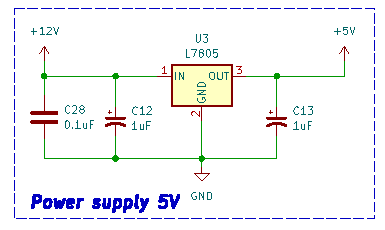
\includegraphics[width=0.6\linewidth]{./my-chapters/my-images/Power_Source/power_supply_5V.pdf}
	\caption{Mạch cung cấp nguồn $+5V$}
	\label{f_supply_+5V}
\end{figure}

Điện áp ngõ vào ($V_{in}$) của mạch cần phải đáp ứng tối thiểu theo công thức: \[ V_{in} > V_{out} + V_{dropout} = 5 + 2 = 7V \rightarrow V_{in} > 7V\]
Trong đó,
\begin{itemize}[label = -]
	\item $V_{in}$: là điện áp đầu vào ($V$).
	\item $V_{out}$: là điện áp đầu ra của LM7805 $=5V$.
	\item $V_{dropout}$: là điện áp rơi trên LM7805 $=2V$.
\end{itemize}

Công suất tiêu tán ($P_{loss}$) là công suất tiêu hao năng lượng dưới dạng nhiệt khi ổn áp: \[ P_{loss} = (V_{in} - V_{out}) \times I_{load} = (12 - 5)\times 1 = 7W\]
Trong đó,
\begin{itemize}[label=-]
	\item $P_{loss}$: là công suất tiêu tán trên LM7805 ($W$).
	\item $V_{in}$: là điện áp ngõ vào LM7805 ($=12V$).
	\item $V_{out}$: là điện áp ngõ ra LM7805 ($=5V$).
	\item $I_{load}$: là dòng tải ($=1A$).
\end{itemize}

Kích thước tản nhiệt ($R_{th}$) để đảm bảo IC không quá nóng, nhiệt độ $T_j$ phải nằm trong giới hạn ($T_j \leq 125^{\circ}C$). Ta sử dụng công thức: \[ T_{j} = T_{o} + P_{loss} \times R_{th(tot)} \rightarrow R_{th(tot)} \leq \dfrac{T_{j} - T_{o}}{P_{loss}} = \dfrac{125 - 25}{7} \approx 14.3 \rightarrow R_{th(tot)} \leq 14.3^{\circ}C/W
\]
\[ \Rightarrow R_{th(c-a)} \leq R_{th(tot)} - R_{th(j-c)} = 14.3 - 5 \rightarrow R_{th(c-a)} \leq 9.3^{\circ}C/W \]
Trong đó,
\begin{itemize}[label = -]
	\item $T_{j}$: là nhiệt độ cho phép hoạt động của IC ($ ^\circ C$).
	\item $T_{o}$: là nhiệt độ của môi trường ($=25^{\circ}C$).
	\item $P_{loss}$: là công suất tiêu tán trên LM7805 ($=7W$).
	\item $R_{th(tot)}$: là tổng trở nhiệt từ junction đến môi trường ($14.3^{\circ}C/W$).
	\item $R_{th(j-c)}$: là trở nhiệt junction-to-case ($=5^{\circ}C/W$).
	\item $R_{th(c-a)}$: là trở nhiệt case-to-air ($^{\circ}C/W$).
\end{itemize}

Tụ điện đầu vào $C_{12}$ giúp bù sụt áp tạm thời và có giá trị là $1\mu F$.

Tụ điện đầu ra $C_{13}$ giúp cải thiện ổn định điện áp đầu ra và có giá trị là $1\mu F$.

Tụ $C_{28}$ là tụ điện có chức năng dập nhiễu cao tần có giá trị là $0.1\mu F$.

Hiệu suất ($\eta$) của mạch được tính bằng công thức: \[ \eta = \dfrac{V_{out}\times I_{load}}{V_{in} \times I_{load}}\times 100\% = \dfrac{5\times 1}{12 \times 1}\times 100\% \approx 41.7\% \]

%\subsection{Điện áp cấp $+3.3V$}
%
%\begin{figure}[H]
%	\centering
%	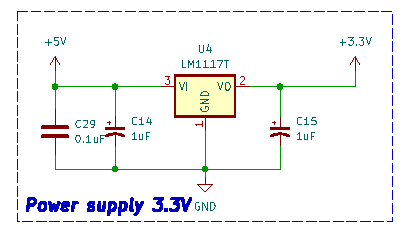
\includegraphics[width=0.6\linewidth]{./my-chapters/my-images/Power_Source/power_supply_3V.pdf}
%	\caption{Mạch cung cấp nguồn $+3.3V$}
%	\label{f_supply_+3.3V}
%\end{figure}
%
%Điện áp ngõ vào ($V_{in}$) của mạch cần phải đáp ứng tối thiểu theo công thức: \[ V_{in} > V_{out} + V_{dropout} = 3.3 + 1.2 = 4.5V \rightarrow V_{in} > 4.5V\]
%Trong đó,
%\begin{itemize}[label = -]
%	\item $V_{in}$: là điện áp đầu vào ($V$).
%	\item $V_{out}$: là điện áp đầu ra của LM117T $=3.3V$.
%	\item $V_{dropout}$: là điện áp rơi trên LM117T $=1.2V$.
%\end{itemize}
%
%Công suất tiêu tán ($P_{loss}$) là công suất tiêu hao năng lượng dưới dạng nhiệt khi ổn áp: \[ P_{loss} = (V_{in} - V_{out}) \times I_{load} = (5 - 3.3)\times 1 = 1.7W\]
%Trong đó,
%\begin{itemize}[label=-]
%	\item $P_{loss}$: là công suất tiêu tán trên LM117T ($W$).
%	\item $V_{in}$: là điện áp ngõ vào LM117T ($=5V$).
%	\item $V_{out}$: là điện áp ngõ ra LM117T ($=3.3$).
%	\item $I_{load}$: là dòng tải ($=1A$).
%\end{itemize}
%
%Kích thước tản nhiệt ($R_{th}$) để đảm bảo IC không quá nóng, nhiệt độ $T_j$ phải nằm trong giới hạn ($T_j \leq 125^{\circ}C$). Ta sử dụng công thức: \[ T_{j} = T_{o} + P_{loss} \times R_{th(tot)} \rightarrow R_{th(tot)} \leq \dfrac{T_{j} - T_{o}}{P_{loss}} = \dfrac{125 - 25}{1.7} \approx 58.8 \rightarrow R_{th(tot)} \leq 58.8^{\circ}C/W
%\]
%\[ \Rightarrow R_{th(c-a)} \leq R_{th(tot)} - R_{th(j-c)} = 58.8 - 2 \rightarrow R_{th(c-a)} \leq 56.8^{\circ}C/W \]
%Trong đó,
%\begin{itemize}[label = -]
%	\item $T_{j}$: là nhiệt độ cho phép hoạt động của IC ($ ^\circ C$).
%	\item $T_{o}$: là nhiệt độ của môi trường ($=25^{\circ}C$).
%	\item $P_{loss}$: là công suất tiêu tán trên LM117T ($=7W$).
%	\item $R_{th(tot)}$: là tổng trở nhiệt từ junction đến môi trường ($58.8^{\circ}C/W$).
%	\item $R_{th(j-c)}$: là trở nhiệt junction-to-case ($=2^{\circ}C/W$).
%	\item $R_{th(c-a)}$: là trở nhiệt case-to-air ($^{\circ}C/W$).
%\end{itemize}
%
%Tụ điện đầu vào $C_{14}$ giúp bù sụt áp tạm thời và có giá trị là $1\mu F$.
%
%Tụ điện đầu ra $C_{15}$ giúp cải thiện ổn định điện áp đầu ra và có giá trị là $1\mu F$.
%
%Tụ $C_{29}$ là tụ điện có chức năng dập nhiễu cao tần có giá trị là $0.1\mu F$.
%
%Hiệu suất ($\eta$) của mạch được tính bằng công thức: \[ \eta = \dfrac{V_{out}\times I_{load}}{V_{in} \times I_{load}}\times 100\% = \dfrac{3.3\times 1}{5 \times 1}\times 100\% = 66\% \]

\subsection{Thực thi mạch nguồn}

\begin{figure}[H]
	\centering
	\begin{minipage}{.45\linewidth}
		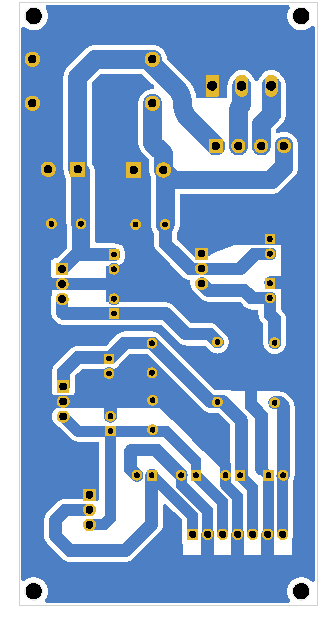
\includegraphics[width=\linewidth]{./my-chapters/my-images/Power_Source/layout_B.pdf}
	\end{minipage}
	\begin{minipage}{.45\linewidth}
		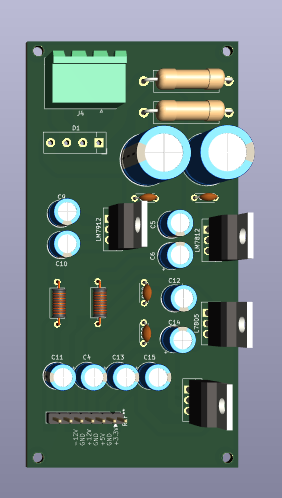
\includegraphics[width=\linewidth]{./my-chapters/my-images/Power_Source/model_3D.png}
	\end{minipage}
	\caption{Thiết kế mạch nguồn.}
\end{figure}

\begin{figure}[H]
	\centering
	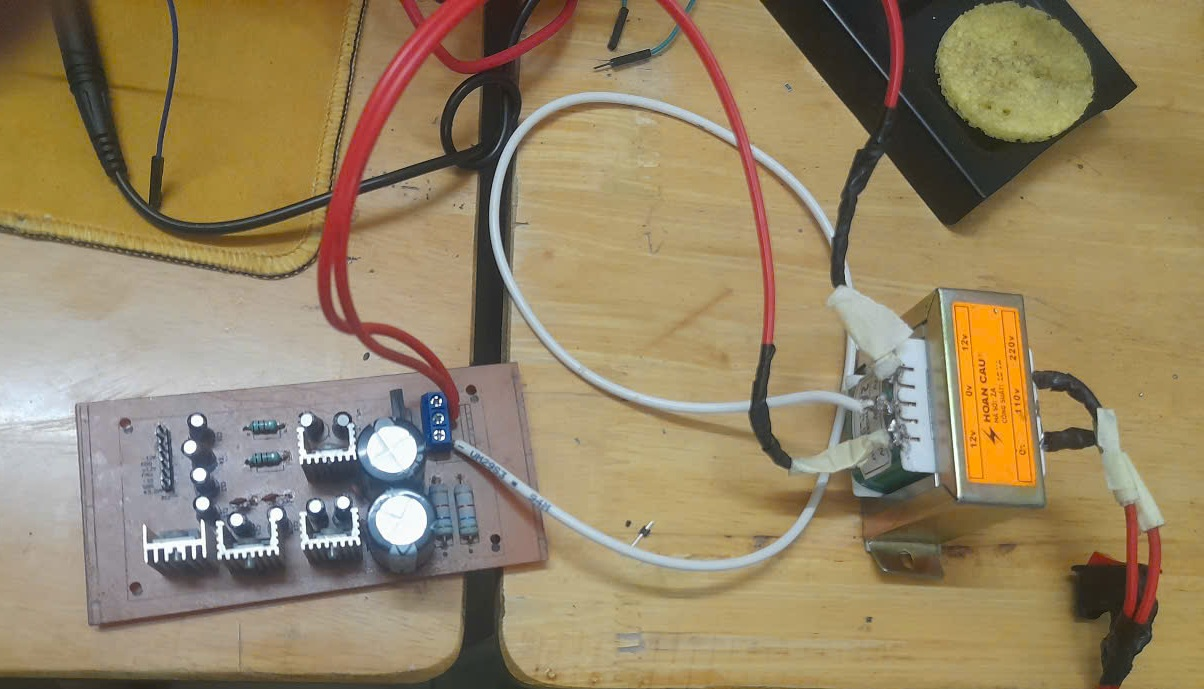
\includegraphics[width=.7\linewidth]{./my-chapters/my-images/Power_Source/mach_thucte.jpg}
	\caption{Hình ảnh thực tế của mạch nguồn.}
\end{figure}

\begin{figure}[H]
	\centering
	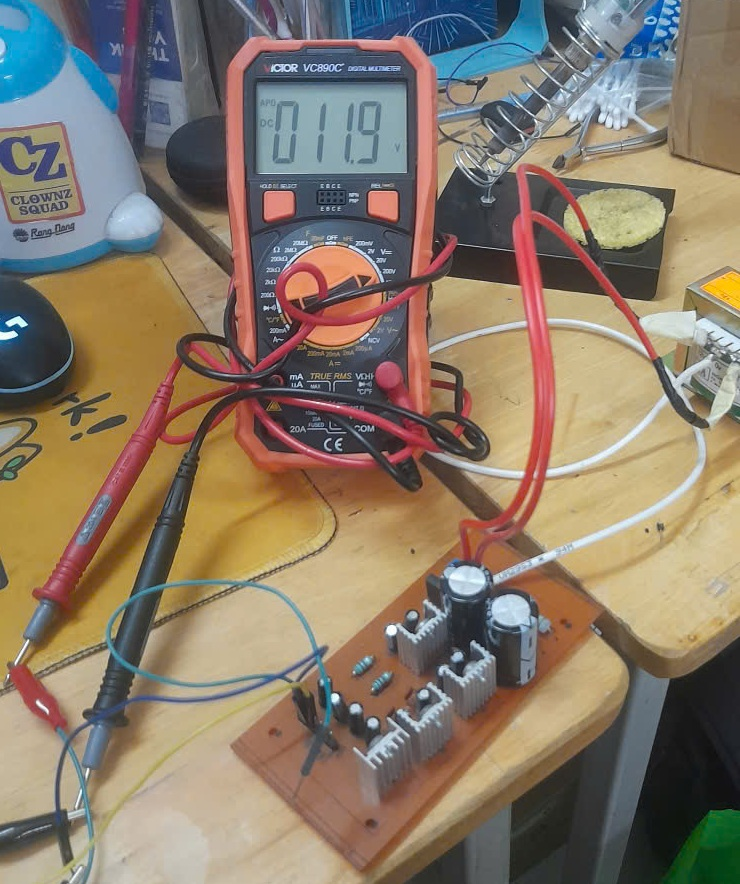
\includegraphics[width=.6\linewidth]{./my-chapters/my-images/Power_Source/thucte_+12V.jpg}
	\caption{Hình ảnh thực tế của mạch nguồn tại $+12V$.}
\end{figure}

\begin{figure}[H]
	\centering
	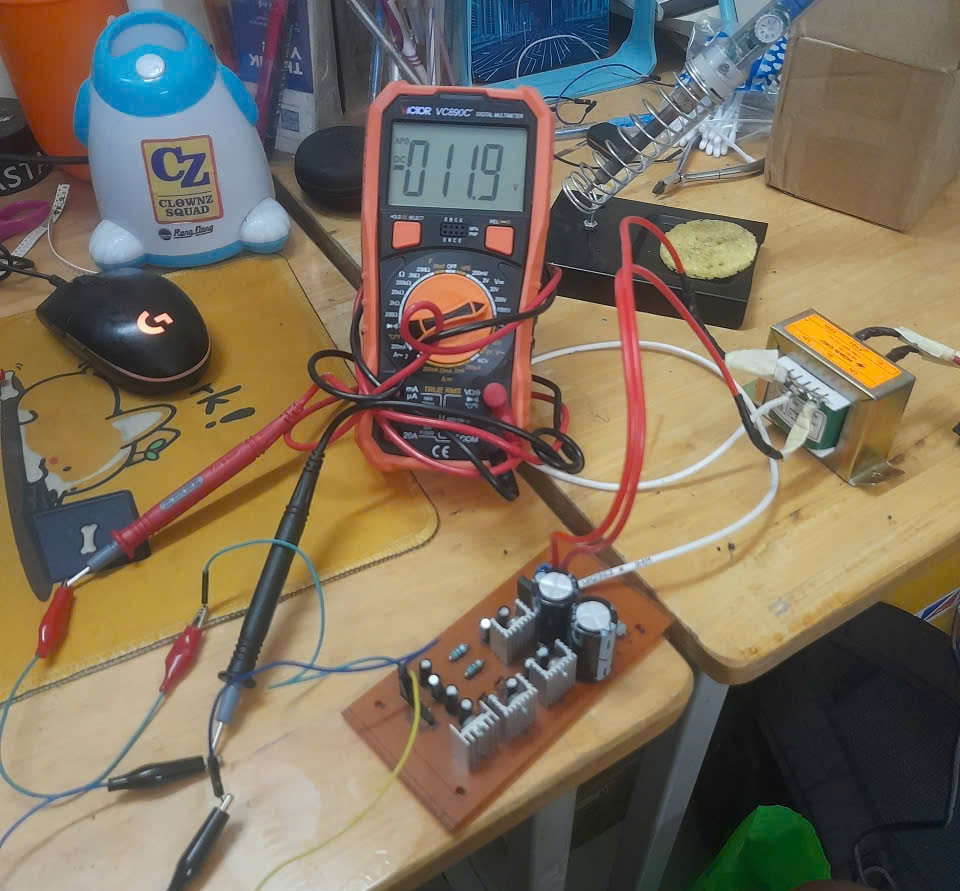
\includegraphics[width=.6\linewidth]{./my-chapters/my-images/Power_Source/thucte_-12V.jpg}
	\caption{Hình ảnh thực tế của mạch nguồn tại $-12V$.}
\end{figure}

\begin{figure}[H]
	\centering
	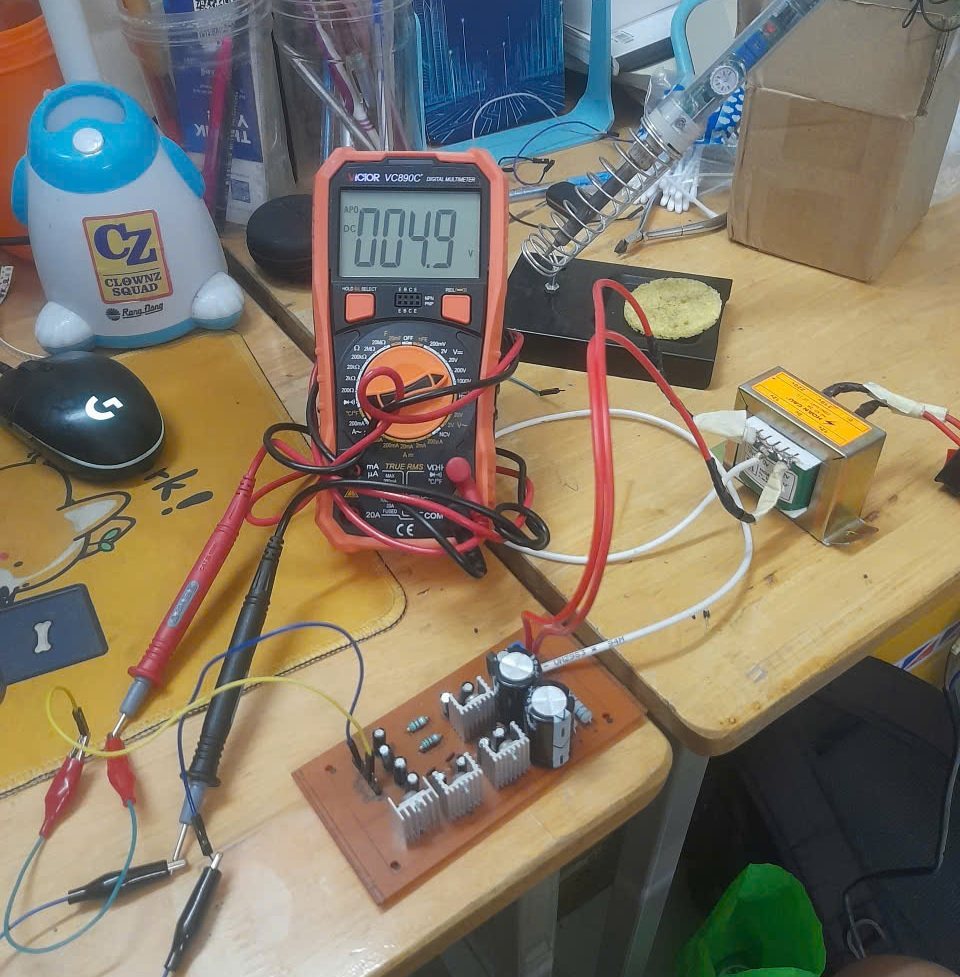
\includegraphics[width=.6\linewidth]{./my-chapters/my-images/Power_Source/thucte_5V.jpg}
	\caption{Hình ảnh thực tế của mạch nguồn tại $+5V$.}
\end{figure}